\documentclass[submit]{harvardml}

% FDV: Check all frontmatter for years, due dates, book sections, etc.
\course{CS181-S23}
\assignment{Assignment \#3}
\duedate{11:59pm EST, March 23rd, 2023}

\usepackage[OT1]{fontenc}
\usepackage[colorlinks,citecolor=blue,urlcolor=blue]{hyperref}
\usepackage[pdftex]{graphicx}
\usepackage{amsmath}
\usepackage{amssymb}
\usepackage{framed}
\usepackage{color}
\usepackage{listings}
\usepackage{enumitem}

\DeclareMathOperator*{\mean}{\mathbb{E}}

\lstset{
  language=Python,
  basicstyle=\ttfamily,
  keywordstyle=\color{blue}\bfseries,
  commentstyle=\color{red},
  stringstyle=\color{green},
  frame=single,
  showstringspaces=false,
}

\definecolor{verbgray}{gray}{0.9}

\lstnewenvironment{csv}{%
  \lstset{backgroundcolor=\color{verbgray},
  frame=single,
  framerule=0pt,
  basicstyle=\ttfamily,
  columns=fullflexible}}{}

\begin{document}

\begin{center}
{\Large Homework 3: Bayesian Methods and Neural Networks}\\
\end{center}

\subsection*{Introduction}

This homework is about Bayesian methods and neural networks. You may want to consider the lecture notes from Feb 14th to 23rd (weeks 4 and 5). Here's an outline of the questions:

\begin{enumerate}
  \item You'll explore the Bayesian paradigm and compare it with the frequentist paradigm for the Beta-Binomial conjugate pair.
  \item You'll derive the backpropagation algorithm for a single-hidden-layer neural network for the binary classification task.
  \item You'll write some code using the PyTorch library for an image classification task.
  \item You'll consider the opportunities and limitations of ML applications and learn to anticipate possible exploits of these systems.
\end{enumerate}

As always, please start early and ask questions on Ed!

Please type your solutions after the corresponding problems using this
\LaTeX\ template, and start each problem on a new page.

Please submit the \textbf{writeup PDF to the Gradescope assignment `HW2'}. Remember to assign pages for each question.  \textbf{You must include your plots in your writeup PDF. } The supplemental files will only be checked in special cases, e.g. honor code issues, etc.

Please submit your \textbf{\LaTeX\ file and code files to the Gradescope assignment `HW2 - Supplemental'}. \\


\newpage

%%%%%%%%%%%%%%%%%%%%%%%%%%%%%%%%%%%%%%%%%%%%%
% Problem 1
%%%%%%%%%%%%%%%%%%%%%%%%%%%%%%%%%%%%%%%%%%%%%

\begin{problem}[Connecting Bayesian and Frequentist Approaches]
  
  In this question, we will gain practice with Bayesian modeling and
  compare it with the frequentist paradigm.
  
  In class, we discussed \emph{Normal-Normal conjugacy.} Now
  we will turn to \emph{Beta-Binomial conjugacy.} This model can be
  visualized in the following way.
  
  You observe a fixed number \(N\) of coin flips (either
  heads or tails) of which \(Y\) (a random variable) are heads. You assume that these are
  drawn by flipping a coin with an unknown probability \(\theta\) of
  landing heads. That is, we choose a \textbf{Binomial likelihood}
  \(Y \sim \mathrm{Bin}(N, \theta)\). The PMF of this distribution is
  given by
  
  \[
  p(Y=y) = {N \choose y} \theta^{y} (1-\theta)^{N-y}.
  \]
  
  \begin{enumerate}
  \item[1.]
    \textbf{Frequentist paradigm and MLE.} The (log) likelihood is all we
    need for frequentist inference. Derive the MLE estimate for \(\theta\)
    given the observations \(Y = y\). That is, find
    \(\arg \max_{\theta} \log p(Y = y \mid \theta)\).
  
  \item[2.]
    \textbf{Beta-Binomial conjugacy.} Under the Bayesian paradigm, we must specify a
    prior distribution for the unknown parameter \(\theta\). We choose a \textbf{Beta prior}
    \(\theta \sim \mathrm{Beta}(\alpha, \beta)\). The PDF of this
    distribution is given by
    
    \[
    p(\theta) \propto \theta^{\alpha - 1} (1-\theta)^{\beta - 1}.
    \]
    
    When the prior and posterior belong to the same distribution family, we
    call the prior-and-likelihood pair a \textbf{conjugate pair.}
    
    \begin{enumerate}
      \item Derive the mean, mode, and variance of the Beta distribution. That is, for $\theta \sim \mathrm{Beta}(\alpha, \beta)$, derive
      
      \begin{enumerate}
        \item $\mean[\theta]$. See hint. \footnote{As an alternative to taking the integral, you may want to use
        \emph{reasoning by representation.} See example 8.5.2 of the Stat 110
        textbook. If you do so, please explain the derivation in your own
        words!}
        \item $\arg \max_{\theta} p(\theta)$ when $\alpha > 1$ and $\beta > 1$. What happens otherwise? (Consider $p(0)$ and $p(1)$.)
        \item $\mathrm{Var}(\theta) = \mean[\theta^2] - (\mean[\theta])^2$.
      \end{enumerate}

      Qualitatively speaking, what does this distribution look like for different $\alpha$ and $\beta$? You can either plot this yourself or see \href{https://en.wikipedia.org/wiki/Beta_distribution}{its Wikipedia page} after deriving the statistics above. What does $\mathrm{Beta}(1, 1)$ correspond to?

      \item 
      Show that the posterior
      \(p(\theta \mid Y=y)\) is indeed Beta and derive its parameters. This proves that a Beta prior and a Binomial likelihood form a conjugate pair; in other words, the Beta distribution is a \textbf{conjugate prior} for the Binomial distribution. See hint.\footnote{For convenience in calculation: Do you need to calculate the normalizing constant? Reuse your results from the previous part.}
    \end{enumerate}
  
\end{enumerate}
\end{problem}

\newpage

\begin{framed}
\begin{enumerate}
  \item[3.]
    \textbf{Posterior mean and mode.} Often we wish to work with just a
    single point estimate of the posterior. Two commonly used point
    estimates are the \emph{posterior mean} and the \emph{posterior mode}
    (a.k.a. the maximum a posteriori (MAP) estimate).
  
    \begin{enumerate}
    \item
      Discuss the advantages and disadvantages of using posterior point
      estimates. Which of these are relevant for our Beta-Binomial conjugate pair? Consider the case when $\alpha, \beta < 1$.
    
    \item
      Using your results from part 2, write down
      
      \begin{enumerate}
        \item the posterior mean estimate \(\theta_{\text{post mean}} = \mean [\theta \mid Y = y]\),
        \item the posterior MAP estimate \(\theta_{\text{MAP}}=\arg \max_{\theta}p(\theta \mid Y=y)\),
        \item and the posterior variance $\mathrm{Var}(\theta \mid Y = y) = \mean[\theta^2 \mid Y = y] - (\mean[\theta \mid Y = y])^2$.
      \end{enumerate}
      
      You shouldn't need any further derivations. That's the nice thing about conjugate priors!
      
    \end{enumerate}

\item[4.]
    \textbf{Prior-posterior connections.}

    \begin{enumerate}
    \item
      Explain in your own words how \(\alpha\) and \(\beta\) affect the
      MAP estimate. How would you set \(\alpha\) and \(\beta\) to reflect
      a prior belief that the coin is fair (i.e.~shows heads and tails
      with equal probability)? (Be careful! See 2.a.ii.)

    \item Now let's analyze the variances of our prior and posterior distributions. Consider the case when $\alpha = \beta$. (If you'd enjoy it, consider the general case for a better understanding.) A sentence or two for each point is fine.
    \begin{enumerate}
      \item How does the variance of the prior relate to the variance of the posterior?
      \item How might you use the prior variance to encode a stronger or weaker prior belief?
      \item How does the posterior variance change as we observe more samples $n$?
    \end{enumerate}
    \end{enumerate}

  \item[5.]
    \textbf{Analysis and connection to frequentism.}
  
    \begin{enumerate}
    \item
      Write a loss function \(\ell(\theta) \in \mathbb{R}\) in terms of
      \(\theta, y, n, \alpha, \beta\) such that minimizing \(\ell\) is
      equivalent to calculating the MAP estimate,
      i.e.~\(\theta_{\text{MAP}} = \arg \min_{\theta} \ell(\theta)\). Your
      function should be a sum of:
      \begin{enumerate}
        \item a mean-squared-error term (which should loosely resemble $(y - \hat y)^2$)
        \item a
        regularization term \(g(\theta) = - a \theta + b \theta^{2}\) for some $a, b$.
      \end{enumerate}
      
      Can you interpret the regularization term? 
      
      Hint: Work backwards from part 1 to derive the MSE term and from part 2.a.ii to get the regularization term. Watch out for the signs! For the interpretation, complete the square and then compare your expression with the prior mode you found in 2.a.ii.
    \item
      What happens to both $\theta_{\text{post mean}}$ and $\theta_{\text{MAP}}$ as \(n \to \infty\)? Compare this to the MLE estimate.
      (Remember to account for the change in \(y\).)
    \end{enumerate}
  
\end{enumerate}

\end{framed}

\subsection*{Solution:}
\begin{enumerate}
    \item  
    $$\arg \max_{\theta} \log p(Y = y \mid \theta) = \arg \max_{\theta} [\log {n\choose y} + y\log (\theta) + (N-y)\log (1-\theta)]$$\\
    To compute this we can take the derivative and set it equal to 0:\\
        \begin{align*}
            \frac{y}{\theta} + (N-y)(-1)\frac{1}{1-\theta} = 0\\
            \frac{y}{\theta} = \frac{N-y}{1-\theta}\\
            \theta N - y\theta = y - y \theta\\
            \boxed{\theta_{MLE} = \frac{y}{N}}
        \end{align*}
    To show that this is a global maximum we will use the second derivative:\\
        \begin{align*}
            \ell''(\theta) = -\frac{y}{\theta^2} - \frac{N-y}{(1-\theta)^2}\\
            \ell''(\theta_{MLE}) = -\frac{N^2}{y} - \frac{N^2}{N-y} < 0
        \end{align*}
    Because this is less than 0 we know we have found a global maximum for our $\theta_{MLE}$\\
    \item
    \begin{enumerate}
        \item $\theta \sim Beta(\alpha, \beta)$\\\begin{enumerate}
            \item 
            % To solve for the expectation we can use the hint to use reasoning by representation just like we did in the Stat 110 textbook. 
            $$E[\theta] = \int_0^1\frac{\Gamma(\alpha + \beta)}{\Gamma(\alpha)\Gamma(\beta)}\theta^{\alpha-1} (1-\theta)^{\beta -1}d\theta$$ 
            We can now apply properties of the Gamma function to simplify this to:\\
            $$= \frac{\Gamma(\alpha + \beta)}{\Gamma(\alpha)} \frac{\Gamma(\alpha + 1)}{\Gamma(\alpha + \beta + 1)}\int_0^1\frac{\Gamma(\alpha + \beta + 1)}{\Gamma(\alpha+1)\Gamma(\beta)}\theta^\alpha (1-\theta)^{\beta -1}d\theta$$
            $$= \frac{\Gamma(\alpha + \beta)}{\Gamma(\alpha)}\cdot \frac{\alpha\Gamma(\alpha)}{(\alpha+\beta)\Gamma(\alpha + \beta)} = \frac{\alpha}{\alpha+\beta}$$\\
            $$\boxed{E[\theta] = \frac{\alpha}{\alpha + \beta}}$$

            \item
            $$\arg \max_{\theta}p(\theta) = \arg \max_{\theta} \theta^{\alpha-1}(1-\theta)^{\beta -1} = \arg \max_{\theta} [(\alpha - 1)\log \theta + (\beta-1)\log(1-\theta)]$$\\
            To compute this we can take the derivative and set it equal to 0.\\
            \begin{align*}
                \frac{\partial}{\partial \theta}[(\alpha - 1)\log \theta + (\beta-1)\log(1-\theta)] &= 0\\
                \frac{\alpha - 1}{\theta} + (\beta -1)(-1)\frac{1}{1-\theta} &= 0\\
                \frac{\alpha - 1}{\theta} &= \frac{\beta -1}{1-\theta}\\
                (\beta -1)\theta &= (\alpha-1)(1-\theta)\\
                \theta(\beta + \alpha -2) &= \alpha -1\\
                \boxed{\theta = \frac{\alpha -1}{\beta + \alpha -2}}
            \end{align*}
            If $\alpha, \beta > 1$ then we know that the beta distribution will be concave so this value for our $\theta_{max}$ must actually be a global maximum. However, if $\alpha, \beta$ are not $> 1$ then we no longer have this guarantee. In this case we would have a PDF that opens upward and is convex (and it is often a bimodal distribution). As a result we would be unable to find the modes by setting the derivative equal to 0.\\
            \item
            $$Var(\theta) = E[\theta^2] - (E[\theta])^2$$\\
            We already know what $E[\theta]$ is from part i) so we just need to calculate $E[\theta^2]$ which we can do very similarly as to how we calculated $E[\theta]$.\\
            $$E[\theta^2] = \int_0^1\frac{\Gamma(\alpha+ \beta + 1)}{\Gamma(\alpha+1)\Gamma(\beta)}\theta^{\alpha}(1-\theta)^{\beta-1}d\theta = \frac{\Gamma(\alpha + \beta)}{\Gamma(\alpha)}\cdot \frac{\Gamma(\alpha + 2)}{\Gamma(\alpha+\beta+2)}\int_0^1\frac{\Gamma(\alpha+ \beta + 2)}{\Gamma(\alpha+2)\Gamma(\beta)}\theta^{\alpha+1}(1-\theta)^{\beta-1}d\theta$$
            $$= \frac{\Gamma(\alpha + \beta)}{\Gamma(\alpha)} \cdot \frac{(\alpha+1)\alpha\Gamma(\alpha)}{(\alpha+\beta+1)(\alpha+\beta)\Gamma(\alpha + \beta)} = \frac{(\alpha+1)\alpha}{(\alpha+\beta+1)(\alpha+\beta)}$$\\
            Using this result we can solve for the variance:\\
            $$Var(\theta) = \frac{(\alpha+1)\alpha}{(\alpha+\beta+1)(\alpha+\beta)} - (\frac{\alpha}{(\alpha+\beta)})^2$$
            $$ = \frac{(\alpha+1)\alpha(\alpha+\beta)}{(\alpha+\beta+1)(\alpha+\beta)^2} - \frac{\alpha^2(\alpha+\beta+1)}{(\alpha+\beta)^2(\alpha+\beta+1)}$$ 
            $$\boxed{Var(\theta) = \frac{\alpha\beta}{(\alpha+\beta)^2(\alpha+\beta+1)}}$$\\
            \\
            Next I looked at this distribution for different values of $\alpha$ and $\beta$. From the graphs we can see that when we change $\alpha$ and $\beta$ the Beta distribution can take many different forms and approximate many other distributions. For example, when $\alpha=2$ and $\beta=8$ the distribution looks similar to an exponential distribution. Additionally, when $\alpha=5$ and $\beta=5$ the distribution kinda looks similar to a Gaussian distribution. We also know that Beta(1,1) is equivalent to the Uniform(0, 1) distribution.\\
        \end{enumerate}
        \item
        We know that the posterior distribution is proportional to the likelihood times the prior:\\
        \begin{align*}
            p(\theta | Y=y) &\propto p(Y=y|\theta)p(\theta)\\
            &= {N\choose y}\theta^y(1-\theta)^{N-y}\cdot \theta^{\alpha -1}(1-\theta)^{\beta-1}\\
            & = {N\choose y}\theta^{y+\alpha -1}(1-\theta)^{N-y+\beta-1}\\
            &\propto \theta^{y+\alpha -1}(1-\theta)^{N-y+\beta-1}\\
        \end{align*}
        Using pattern matching we know that this is also a Beta distribution with $a= y+\alpha$ and $b=N+\beta - y$:\\
        $$\boxed{p(\theta|Y=y) \sim Beta (y+\alpha, N+\beta - y)}$$
    \end{enumerate}
    \item
    \begin{enumerate}
        \item One of the main advantages of using posterior point estimates is that we are able to use our model to make a single prediction (which is often necessary in the real world). However, using posterior point estimates can also have many disadvantages. For example, both the posterior mean and posterior mode can sometimes be misleading to use. Sometimes the posterior mode will be an exception point (the posterior is highest at posterior mode but the points very close to posterior mode are considered very unlikely). Similarly, sometimes the posterior mean is an unlikely point. Ultimately, these values can be deceiving because we cannot see the uncertainty around this point.\\
        \\
        For the Beta-Binomial conjugate pair posterior point estimates can be useful because we are actually able to compute our posterior distribution (because we have a conjugate pair). As a result the posterior MAP can be useful because we are able to compute the maximum likelihood. However, in the case when $\alpha, \beta < 1$, there does not exist a MAP estimate because our distribution is no longer concave so we can no longer find a global maximum (as we showed in question 2.a.ii). This means that we cannot use the MAP to calculate a posterior point estimate, but we can use the posterior mean instead. \\
        \item
        \begin{enumerate}
        In part 2.a.i we found an equation for the expectation of a Beta distribution. We can use this equation here:\\
            \item $$\boxed{\theta_{\textnormal{post mean}} = E[\theta | Y=y] = \frac{y+\alpha}{\alpha + N + \beta}}$$
        \\
        \item
        Assuming $y+\alpha, N+\beta-y >1:$\\
        $$\theta_{\textnormal{MAP}} = \arg \max_{\theta}p(\theta |Y=y) = \arg \max_{\theta}[\theta^{y+\alpha -1}(1-\theta^{N-y+\beta-1})]$$
        \begin{align*}
           \frac{\partial}{\partial \theta}[(y+\alpha-1)\log(\theta) + (N-y+\beta -1)\log(1-\theta)] = 0\\
           \frac{y+\alpha -1}{\theta} = \frac{N-y+\beta -1}{1-\theta}\\
           (1-\theta)(y+\alpha -1) = \theta (N-y+\beta -1)\\
           \boxed{\theta_{\textnormal{MAP}} = \frac{y+\alpha -1}{N+\beta + \alpha -2}}
        \end{align*}\\
        \item
        Using the formula we found in 2.a.iii we can solve for the variance of this Beta distribution:\\
        $$\boxed{Var(\theta|Y=y) = \frac{(y+\alpha)(N+\beta -y)}{(\alpha + N + \beta)^2(\alpha + N + \beta +1)
        )}}$$\\
        \end{enumerate}
    \end{enumerate}
    \item
        \begin{enumerate}
            \item We know from above that our MAP estimate is equal to: $\theta_{\textnormal{MAP}} = \frac{y+\alpha -1}{N+\beta + \alpha -2}$\\
            This means that if $\alpha$ is really large then our MAP will get really close to 1 (a really high chance of landing on heads) and if $\beta$ is really large then our MAP will tend towards 0 (a higher chance of landing on tails). \\In order to reflect a prior belief that the coin is fair we would want to set $\alpha = \beta$. If we plugged this into our value of $\theta$ that we found in 2.a.ii we would see $\theta = \frac{\alpha-1}{2\alpha-2} = \frac{1}{2}$. This would mean that the probability of drawing a heads is $\frac{1}{2}$ so the probability of drawing tails is also $\frac{1}{2}$\\
            \item
            \begin{enumerate}
                \item 
                We can first calculate the variance of the prior and the posterior when $\alpha = \beta$:\\
            Prior variance = $\frac{\alpha^2}{(2\alpha)^2(2\alpha + 1)}$\\
            Posterior variance = $\frac{(y+\alpha)(N+\alpha -y)}{(2\alpha+N)^2(2\alpha + N + 1)}$\\
            \\
            We can clearly see that asymptotically both of these equations will become $\frac{1}{\alpha}$. This means that as the prior variance decreases, the posterior variance will also decrease.\\
            \item
            We know that a smaller prior variance means we have a stronger prior belief. This means that if we increase our prior variance we can encode a weaker prior belief, and if we decrease our prior variance, we can encode a stronger prior belief. In order to increase our posterior variance we want to decrease $\alpha$.\\
            \item 
            From the equation of our posterior variance we can see that as $N$ increases our posterior variance decreases. This means that as the number of samples increase our posterior variance decreases indicating that we are more certain.\\
            \end{enumerate}
            
        \end{enumerate}
        \item
        \begin{enumerate}
            \item 
            We can first write a generalized loss function:\\
            $$\ell(\theta)=(y-\hat{y})^2+g(\theta) = (y-\hat{y})^2-a\theta+b\theta^2$$\\
            We can then rewrite this using our MSE for this model:\\
            $$\ell(\theta) = \frac{1}{2N}(y-N\theta)^2-a\theta+b\theta^2$$\\
            Now we want to find the values of $a$ and $b$ such that minimizing $\ell$ is equivalent to calculating the MAP estimate. In order to do this we will take the derivative of this loss function and compare it with the value of $\theta_{\textnormal{MAP}}$ that we found above.\\
            $$\frac{\partial \ell}{\partial \theta} = \frac{1}{2N}(2)(y-N\theta)(-N)  - a +2b\theta = 0$$
            $$-y + N\theta - a + 2b\theta = 0$$
            $$\theta(N+2b) = y + a$$
            $$\theta = \frac{y+a}{N+2b} = \theta_{\textnormal{MAP}} = \frac{y+\alpha-1}{N+\beta + \alpha-2}$$\\
            Now we can do some pattern matching in order to solve for $a$ and $b$:\\
            $a = \alpha -1$\\
            $b = \frac{1}{2}(\beta + \alpha -2)$\\
            This means our loss function is equal to:\\
            $$\boxed{\ell(\theta) = \frac{1}{2N}(y-N\theta)^2-(\alpha-1)\theta + \frac{1}{2}(\beta+\alpha -2)\theta^2}$$
            Now in order to interpret this regularization term we can complete the square on the regularization term:\\
            \begin{align*}
                g(\theta) &= -(\alpha - 1)\theta + \frac{1}{2}(\alpha + \beta -2)\theta^2\\
                &= \frac{1}{2}(\beta+\alpha-2)(\theta^2-2\cdot\frac{\alpha-1}{\beta+\alpha-2}\cdot \theta)\\
                &=\frac{1}{2}(\beta+\alpha-2)(\theta^2 - 2M\theta + M^2 -M^2) \textnormal{ where } M = \frac{\alpha-1}{\beta+\alpha-2}\\
                &=\frac{1}{2}(\beta+\alpha-2)(\theta-M)^2-\frac{1}{2}(\beta+\alpha-2)M^2
            \end{align*}
            From the first term we can see that our regularization term is pushing our value of $\theta$ towards our value of $M$. Interestingly, we can see that our value of $M$ is actually equal to the prior mode we found in part 2.a.ii. This means that our regularization term is penalizing values of $\theta$ that are farther away from our prior mode. Overall, this means that our regularization is adding even more weight to our prior and adding more bias.\\
            % $\frac{\alpha-1}{\beta+\alpha-2}$
            \item
            We know that our $\theta_{\textnormal{post mean}}$ is equal to:
            $$\theta_{\textnormal{post mean}} = E[\theta | Y=y] = \frac{y+\alpha}{\alpha + N + \beta}$$
            This means that as $N \rightarrow \infty$ our post mean goes towards: $\boxed{\frac{y}{N}}$\\
            Similarly, our $\theta_{\textnormal{MAP}}$ is equal to:\\
            $$\theta_{\textnormal{MAP}} = \frac{y+\alpha-1}{N+\beta + \alpha-2}$$
            So as $N \rightarrow \infty$, our MAP also tends towards $\boxed{\frac{y}{N}}$\\
            \\
            Furthermore, we found in part a that our MLE estimate is also equal to $\boxed{\frac{y}{N}}$
        \end{enumerate}
\end{enumerate}

\newpage

%%%%%%%%%%%%%%%%%%%%%%%%%%%%%%%%%%%%%%%%%%%%%
% Problem 2
%%%%%%%%%%%%%%%%%%%%%%%%%%%%%%%%%%%%%%%%%%%%%

\begin{problem}[Neural Networks]

    In this problem, we will take a closer look at how gradients are calculated for backprop with a simple multi-layer perceptron (MLP). The MLP will consist of a first fully connected layer with a sigmoid activation, followed by a one-dimensional, second fully connected layer with a sigmoid activation to get a prediction for a binary classification problem. We use non-linear activation functions as the composition of linear functions is linear. Assume bias has not been merged. Let:
    \begin{itemize}
        \item $\bold{W}_1$ be the weights of the first layer, $\bold{b}_1$ be the bias of the first layer.
        \item $\bold{W}_2$ be the weights of the second layer, $\bold{b}_2$ be the bias of the second layer.
    \end{itemize}
    
    The described architecture can be written mathematically as: $$\hat{y} = \sigma(\bold{W}_2 \left[\sigma \left(\bold{W}_1 \bold{x} + \bold{b}_1\right)\right] + \bold{b}_2)$$
    
    where $\hat{y}$ is a scalar output of the net when passing in the single datapoint $\bold{x}$ (represented as a column vector), the additions are element wise additions, and the sigmoid is an element wise sigmoid.
    
    \begin{enumerate}
        \item Let:
        \begin{itemize}
            \item $N$ be the number of datapoints we have
            \item $M$ be the dimensionality of the data
            \item $H$ be the size of the hidden dimension of the first layer. Here, hidden dimension is used to describe the dimension of the resulting value after going through the layer. Based on the problem description, the hidden dimension of the second layer should be 1.
        \end{itemize}
        
        Write out the dimensionality of each of the parameters, and of the intermediate variables:
  
            \begin{align*}
            \bold{a}_1 &= \bold{W}_1 \bold{x} + \bold{b}_1, 
            &\bold{z}_1 = \sigma(\bold{a}_1) \\
            a_2 &= \bold{W}_2 \bold{z}_1 + \bold{b}_2, 
            &\hat{y} = z_2 = \sigma(a_2)
            \end{align*}
            
        and make sure they work with the mathematical operations described above. Examining shapes is one of the key ways to debug your code, and can be done using .shape after any numpy array.
        
        \item  We will derive the gradients for each of the parameters, which can then be used along with gradient descent to find weights that improve our model's performance. For this question, assume there is only one datapoint $\bold{x}$, and that our loss is $L = -(y \log (\hat{y}) + (1 - y) \log (1 - \hat{y}))$. For all questions, the chain rule will be useful.
      \begin{enumerate}
          \item Find $\frac{\partial L}{\partial b_2}$. 
          
          \item Find $\frac{\partial L}{\partial W_2^h}$, where $W_2^h$ represents the $h$th element of $\bold{W}_2$.
          
          \item Find $\frac{\partial L}{\partial b_1^h}$, where $b_1^h$ represents the $h$th element of $\bold{b}_1$. (*Hint: Note that only the $h$th element of $\bold{a}_1$ and $\bold{z}_1$ depend on $b_1^h$ - this should help you with how to use the chain rule.)
          
          \item Find $\frac{\partial L}{\partial W_1^{h,m}}$, where  $W_1^{h,m}$ represents the element in row $h$, column $m$ in $\bold{W}_1$.
      
      \end{enumerate}

\end{enumerate}

\end{problem}

\newpage 

\begin{framed}
    \noindent\textbf{Problem 2} (cont.)\\
    \begin{enumerate}
    \setcounter{enumi}{2}
    
      \item  We now explore an example of forward-mode auto-differentiation. Consider the following 
          equation:
    
          $$
            f(x_1, x_2) = \ln (\sin (x_1)) + x_1 \exp \{ x_2 \}
          $$
    
          This equation can be split up using intermediate variables $v_1, \dots, v_7$ as follows:
    
          \begin{align*}
            v_1 &= x_1 \\ 
            v_2 &= \sin (v_1) \\
            v_3 &= \ln (v_2) \\
            v_4 &= x_2 \\
            v_5 &= \exp \{ v_4 \} \\
            v_6 &= v_1v_5 \\
            v_7 &= v_3 + v_6 \\
            f(x_1, x_2) &= v_7
          \end{align*}
    
            Splitting up the equation like this is very similar to what an auto-differentiation 
            library would do. From these equations we can construct a \textit{computational graph} 
            where each node of the graph corresponds to an input, an intermediate variable, or 
            the output. 
    
        \begin{enumerate}
            \item Let $x_1 = \frac{\pi}{6}$ and $x_2 = 1$. Calculate the values of all the 
                intermediate variables $v_1, \dots v_7$ and $f(x_1,x_2)$. 
            \item Calculate the derivative of
                all of the intermediate variables $v_1, \dots, v_7$ and
                $f$ with respect to $x_1$ evaluated 
                at $x_1 = \frac{\pi}{6}$ and $x_2 = 1$.  
    
        \end{enumerate}
    
    \item \textbf{Extra Credit (Hard):} Consider two neural networks $f_1$ and $f_2$ for binary 
        classification. They each take in inputs $x \in \mathbb{R}^2$ and output a 
        prediction $\hat{y} \in [0,1]$. $f_1$
        consists of a single hidden layer with 4 nodes, each with 
        a ReLU activation function. These nodes are connected to a single sigmoid output node. Thus 
        $f_1$ has the following form:
    
        $$
        f_1(x) = \sigma\left( W_2[ReLU(W_1 x + b_1)] + b_2 \right)
        $$
    
        $f_2$ consists of 2 hidden layers, each with 2 ReLU activated nodes. Just as in $f_1$, the 
        nodes of the final layer are connected to a single sigmoid output node. 
        Thus $f_2$ has the following form:
    
        $$
        f_2(x) = \sigma(W_3[ReLU(W_2[ReLU(W_1 x + b_1)]+b_2)]+ b_3)
        $$
    
        We leave finding the shapes of the weight and bias vectors up to you, noting that 
        by convention $x$ should be considered a column vector with 2 elements. 
    
        Draw a classification boundary that $f_2$ can express but $f_1$ cannot and argue 
        why $f_2$ can express the boundary but $f_1$ cannot.
    
    
    \end{enumerate}  
\end{framed}

\subsection*{Solution:}
\begin{enumerate}
    \item 
    $W_1: H \times M$\\
    $x: M \times 1$\\
    $b_1 : H \times 1$\\
    $a_1 : H\times 1$\\
    $z_1 : H\times 1$\\
    $W_2 : 1 \times H$\\
    $b_2 : 1 \times 1$\\
    $a_2 : 1 \times 1$\\
    $\hat{y} = z_2 : 1 \times 1$\\
    \item
    \begin{enumerate}
        \item 
        \begin{align*}
            \frac{\partial L}{\partial b_2} =& \frac{\partial L}{\partial \hat{y}} \cdot \frac{\partial \hat{y}}{\partial a_2} \cdot \frac{\partial a_2}{\partial b_2}\\
            =& - (\frac{y}{\hat{y}} + (1-y)(-1)\frac{1}{1-\hat{y}})\cdot \hat{y}(1-\hat{y})\\
            =&-(\frac{y}{\hat{y}} - \frac{1-y}{1-\hat{y}})\hat{y}(1-\hat{y})\\
            =&\hat{y}y - y + \hat{y}  - y\hat{y} = \boxed{\hat{y}-y}
        \end{align*}
        \item
        \begin{align*}
            \frac{\partial L}{\partial W_2^h} =& \frac{\partial L}{\partial \hat{y}} \cdot \frac{\partial \hat{y}}{\partial a_2} \cdot \frac{\partial a_2}{\partial W_2^h}
            = \boxed{(\hat{y}-y)\cdot z_1^h} 
        \end{align*}
        \item
        \begin{align*}
            \frac{\partial L}{\partial b_1^h} =& \frac{\partial L}{\partial \hat{y}} \cdot \frac{\partial \hat{y}}{\partial a_2} \cdot \frac{\partial a_2}{\partial z_1^h} \cdot
            \frac{\partial z_1^h}{\partial a_1^h} \cdot
            \frac{\partial a_1^h}{\partial b_1^h}\\
            =&(\hat{y}-y)\cdot W_2^h \cdot z_1^h (1-z_1^h) \cdot 1\\
            &\boxed{(\hat{y}-y)\cdot W_2^h \cdot z_1^h (1-z_1^h)}
        \end{align*}
        \item
        \begin{align*}
            \frac{\partial L}{\partial W_1^{h,m}} =& \frac{\partial L}{\partial \hat{y}} \cdot \frac{\partial \hat{y}}{\partial a_2} \cdot \frac{\partial a_2}{\partial z_1} \cdot
            \frac{\partial z_1^h}{\partial a_1^h} \cdot
            \frac{\partial a_1^h}{\partial W_1^{h,m}}\\
            &\boxed{(\hat{y}-y)\cdot W_2^h \cdot z_1^h (1-z_1^h)\cdot x^m}
        \end{align*}
    \end{enumerate}
    \item
    \begin{enumerate}
        \item 
        \begin{align*}
            v_1 = \frac{\pi}{6}\\
            v_2 = \sin(\frac{\pi}{6}) = \frac{1}{2}\\
            v_3 = \ln(\frac{1}{2})\\
            v_4 = 1\\
            v_5 = e\\
            v_6 = \frac{\pi}{6}e\\
            v_7 = \ln(\frac{1}{2}) + \frac{\pi}{6}e = f(x_1, x_2)\\
        \end{align*}
        \item
        \begin{align*}
            \frac{\partial v_1}{\partial x_1} = 1\\
            \frac{\partial v_2}{\partial x_1} = \cos(x_1) = \cos(\frac{\pi}{6}) = \frac{\sqrt{3}}{2}\\
            \frac{\partial v_3}{\partial x_1} = \frac{1}{v_2}\cdot\frac{\partial v_2}{\partial x_1} = \frac{1}{\sin(\pi/6)}\cdot \cos(\pi/6) = \frac{1}{\tan(\pi/6)} = \sqrt{3}\\
            \frac{\partial v_4}{\partial x_1} = 0\\
            \frac{\partial v_5}{\partial x_1} = \frac{\partial v_4}{\partial x_1}\cdot \frac{1}{v_4} = 0\\
            \frac{\partial v_6}{\partial x_1} = \frac{\partial v_5}{\partial x_1}\cdot v_1 + \frac{\partial v_1}{\partial x_1} \cdot v_5 = 0 + exp(x_2) = e^1 = e\\
            \frac{\partial v_7}{\partial x_1} = \frac{\partial v_3}{\partial x_1} + \frac{\partial v_6}{\partial x_1} = \sqrt{3} + e\\
        \end{align*}
    \end{enumerate}
    \item Extra Credit Attempt\\
    I will begin thinking about this problem by first trying to understand exactly what the ReLU function is doing. We know that if the value inputted into the ReLU function is less than 0 then ReLU will output 0 but if the input is greater than 0 then ReLU will just return the input. Thus we can almost think of the ReLU as a division boundary. On one side of the boundary are all the 0's (negative inputs) and on the other side of the boundary are all the positive inputs (we can consider these to be 1's). \\
    \\
    Now we can look more closely at $f_2$ which consists of 2 hidden layers. In this function we are taking a ReLU of a ReLU. As a result, rather than thinking about creating one division boundary we are creating 4. It is almost as if we are creating 4 quadrants. \\
    \\
    Now that we have thought about what exactly $f_1$ and $f_2$ are doing we can find a classification boundary that $f_2$ can express but $f_1$ cannot. We need some sort of boundary that needs more than 2 quadrants (we need 4).
    
\end{enumerate}


\newpage

%%%%%%%%%%%%%%%%%%%%%%%%%%%%%%%%%%%%%%%%%%%%%
% Problem 3
%%%%%%%%%%%%%%%%%%%%%%%%%%%%%%%%%%%%%%%%%%%%%

\begin{problem}[Modern Deep Learning Tools: PyTorch]

In this problem, you will learn how to use PyTorch. This machine learning library is massively popular and used heavily throughout industry and research. 


\begin{enumerate}
    \item In \verb|T3_P3.ipynb| you will implement an MLP for image classification from scratch. Paste your code solutions below and include a final graph of your training progress. Also submit your completed \verb|T3_P3.ipynb| file.
    \item Discuss what trends you see with your plot (train/test loss and train/test accuracy).
\end{enumerate}

\textbf{Out of Distribution (OOD) Analysis}: Now, let's evaluate the usefulness of the predictive uncertainties of our model for test data that are dissimilar to our training data. These test data points are called out of distribution (OOD) points. Just as in Homework 2, we want the predictive uncertainties from our models to help us distinguish in-distribution test data (test data that are similar to data on which we trained our model) and OOD test data. Again, in many safety-critical applications of ML, we want human-experts to override model decisions if the model is operating on extremely unfamiliar data. 

\hspace{3mm} 3. Report both the in and out distribution test accuracies of your model. In a couple of sentences, discuss what you notice about these accuracies.

  {\bfseries You will recieve no points for code not included below.}

  {\bfseries You will recieve no points for code using built-in APIs from the \verb|torch.nn| library.}
  
\end{problem}


\subsection*{Solution:}

Plot:

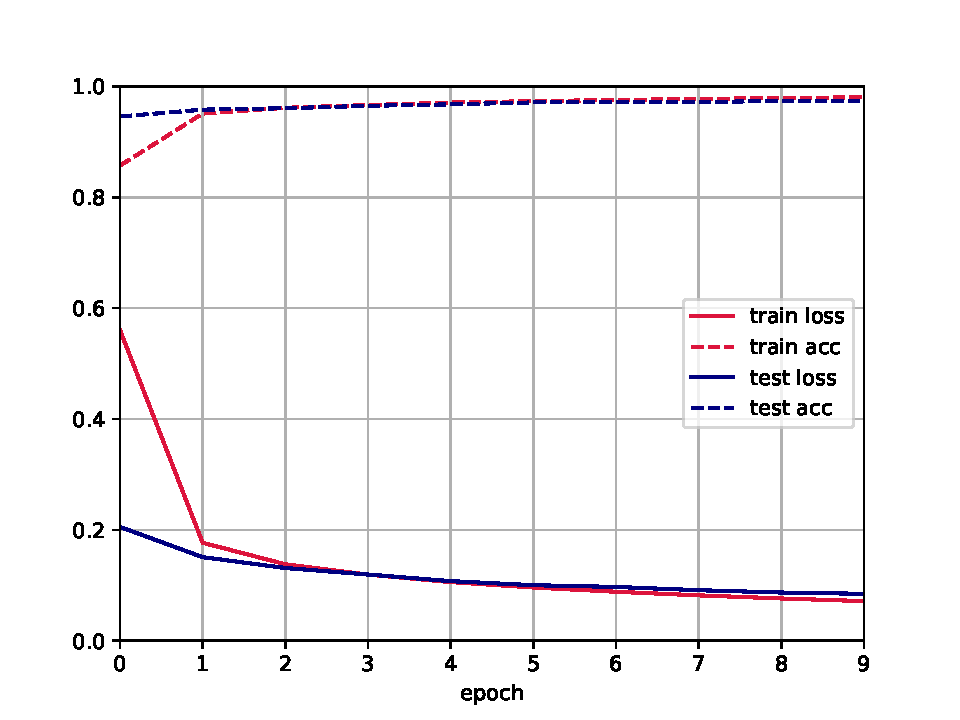
\includegraphics[width=\linewidth]{final_plot}

Code:

\begin{lstlisting}[language=Python]
n_inputs = 28*28
n_hiddens = 256
n_outputs = 10 

W1 = torch.nn.Parameter(0.01*torch.randn(size=(n_inputs, n_hiddens))) 
b1 = torch.nn.Parameter(torch.zeros(n_hiddens))
W2 = torch.nn.Parameter(0.01*torch.randn(size=(n_hiddens, n_outputs))) 
b2 = torch.nn.Parameter(torch.zeros(n_outputs)) 


def relu(x):
    return torch.clamp(x, min=0)



def softmax(x):
    var = torch.exp(X)
    sums = torch.sum(var, dim=1, keepdim=True)
    return var/sums



def net(X):
  X = X.flatten(start_dim=1)
  H = relu(X @ W1 + b1)
  O = softmax(H@W2 + b2)
  return O



def cross_entropy(y_hat, y):
  return -torch.log(y_hat[range(len(y_hat)), y])



def sgd(params, lr=0.1):
  with torch.no_grad():
    for param in params:
        param -= lr*param.grad
        param.grad.zero_()



def train(net, params, train_iter, loss_func=cross_entropy, updater=sgd):
  epochs = 10
  
  for epoch in range(epochs):
    for X, y in train_iter:
      
      # Calculate y_hat from X
      y_hat = net(X)
    
      # Calculate total loss
      l = loss_func(y_hat, y).mean()

      # Backpropagate on the loss
      l.backward()
        
      # Update parameters with SGD  
      updater(params)

\end{lstlisting}
\begin{enumerate}
    \item Pasted above
    \item Looking at the plot pasted above we can clearly see trends in the test/train accuracy and test/train loss. Let's first analyze the accuracy. At epoch 0 we see that the neural network is learning which is why the test / train accuracy is not nearly as close to 1.0 as in the later epochs. However, as we move through each epoch both the train and test accuracy's get closer and closer to 1.0 meaning the model is being trained and getting more accurate. Similarly when looking at the train/test losses we can see that at the beginning (when the model is still learning) the losses are much higher but as we move through the epochs the loss gets closer to zero. Interestingly we see that this model learns very quickly. It only takes about 1 epoch for the train and test lines to converge and the initial jump is very large whereas the later increases in accuracy and decreases in loss are much smaller.\\
    \item
    Test Accuracy (In Distribution): 0.9967830882352942\\
    Test Accuracy (Out of Distribution): 0.34123149514198303\\
    \\
    Our test accuracy in distribution is very very high (rounds to 1.0) whereas the test accuracy out of distribution is much much lower (less than 0.5). These results follow very closely with what we discussed in lecture about in and out of distribution data. Data that is in distribution is very similar to the data that our model is trained on which is why our model is very good at making predictions. Out of distribution test data is unlike our training data which is why our model cannot predict as well and will be less accurate.
\end{enumerate}

%%%%%%%%%%%%%%%%%%%%%%%%%%%%%%%%%%%%%%%%%%%%%
% Problem 4
%%%%%%%%%%%%%%%%%%%%%%%%%%%%%%%%%%%%%%%%%%%%%

\begin{problem}[Impact Question: Testing security of neural networks deployed in autonomous vehicles and suggesting policy recommendations (9 points)]

\textbf{The learning goal of the impact questions of this homework is
three-fold: }

\begin{enumerate}
\item
  Get trained in adversarial thinking to be able to anticipate risks and
  possible exploits when designing Machine Learning applications
\item
  Understand opportunities and limitations to safety and security of
  Machine Learning applications
\item
  Learn to put yourself in the shoes of policymakers who are in charge
  of ensuring safety of real-world Machine Learning applications.
\end{enumerate}

\textbf{Prompt: }You are the Director of Machine Learning of the US
Department of Transportation (a federal US government agency).

The Secretary of the US Department of Transportation declares security
of Machine Learning applications deployed in autonomous vehicles as one
of the priorities of the agency. You are tasked to assess the security
of Machine Learning systems deployed in autonomous vehicles and develop
policy recommendations for the US Department of Transportation.

\textbf{Context: }Tesla employs Neural Networks for perception and
control tasks: For example semantic segmentation, object detection and
monocular depth estimation is performed by Neural Networks on images
captured with the car's camera system to identify road signs, traffic
lights, pedestrians, cars or other traffic related individuals,
vehicles, and objects. The full build autopilot consists of more than 48
networks which must identify high-risk scenarios and provide robust
predictions to ensure safety.

Moreover, beyond cameras Tesla also uses additional sensor systems such
as LiDAR or ultrasonic sensors. Yet, Tesla's engineering and design
approaches are still iterated and their software gets updated.

Link to a demo video: \url{https://tesla-cdn.thron.com/static/NGSLYL_network_XZCUMR.mp4}

Please answer the questions below by using concise language (350 - 700
words in total). Bullet points are appropriate.

\textbf{Questions: }

\begin{enumerate}
\item
  \textbf{Adversarial thinking: }List and explain 3 options how you
  could attack the Neural Network deployed in a self-driving car to make
  it crash. In particular, explain the impact of the attack on the
  statistical properties of input data and predictions of the Neural
  Network. (3 points)

  \begin{enumerate}
  \item
    \textbf{Hardware adversarial attack: }List and explain one attack
    which targets the hardware system of an autonomous vehicle or its
    physical surround.
  \item
    \textbf{Software adversarial attack:} List and explain one attack
    which targets the software system of an autonomous vehicle.
  \item
    \textbf{Social engineering:} List and explain one attack which
    relies on social engineering to make an autonomous vehicle crash.
  \end{enumerate}

\item
  \textbf{Safeguards: }For each of the 3 attack options that you listed
  above, suggest and explain one possible solution that could safeguard
  the Neural Network deployed in Tesla's autopilot. (3 points)

\item
  \textbf{Policy recommendation: }The Secretary of the US Department of
  Transportation asks you to develop one policy recommendation on how to
  ensure sufficient security of deployed neural networks in autonomous
  vehicles.

  \begin{enumerate}
  \item
    \textbf{Recommendation:} List and explain one policy recommendation
    that the US Department of Transportation should implement. (1 point)
  \item
    \textbf{Benefit: }List and explain one benefit of your chosen
    recommendation. (1 point)
  \item
    \textbf{Drawback: }List and explain one drawback of your chosen
    recommendation. (1 point)
  \end{enumerate}
\end{enumerate}

\end{problem}

\newpage

\subsection*{Solution:}
\begin{enumerate}
    \item 
    \begin{enumerate}
        \item One way to attack the hardware system of an autonomous vehicle is to attack the car's camera system that is used to view road signs, traffic lights, pedestrians, etc. One way to do this would be to break the glass on the camera so that it cannot capture clear pictures of its surroundings. If the pictures are not clear then the neural networks cannot interpret the car's surroundings (or might interpret them incorrectly) which could lead to car accidents, injuries, and deaths.\\
        % \item One way to attack the software system of an autonomous vehicle is to attack the software within the sensors that the car uses. We could alter the software so that there is a delay whenever something new is perceived which would prevent the car from reacting fast enough. For example, if a bicycle passing a car is perceived by the sensor but there is a delay then the car might begin to turn without realizing the bicycle is on its side causing the car to hit the bike.\\
        \item In a software adversarial attack, we are aiming to attack the model itself. One way to do this on an autonomous vehicle is to mess with the neural network models by introducing new OOD data into the model. For example, a model focused on autonomous cars would typically be focused on identifying pedestrians, cars, road signs, lane lines, etc., but if we were to feed the model an image of a road sign with a star on it, it would be very confused and struggle to identify it (as the model was not trained on images like this). As a result, the car might behave in a strange way putting the driver as well as others around the car in danger.\\
        \item A social engineering attack will aim to exploit loopholes or other weaknesses in the human portion of decision making. As a result, in order to attack an autonomous vehicle using social engineering one could send phishing emails to Tesla employees. The email could contain a bug so that when the employees open the email, the hacker is able to gain control over Tesla systems. It could then use this control to alter the software of the autonomous vehicles so that they do not behave as they should.\\
    \end{enumerate}
    \\
    \item
    \begin{enumerate}
        \item One possible way to safeguard the cameras used in the Neural Network deployed in Tesla's autopilot is to prioritize protecting the car's cameras. They can be hidden within the car and surrounded by extra protective glass so that an intruder would not be able to find or break the cameras. \\
        % \item One way to safeguard against the software attack that I explained above would be to add several levels of security around the Tesla software so that it cannot be hacked and altered. Tesla can make it so that Tesla car owners can only update their software by going to a Tesla location and having a Tesla employee conduct the update. Furthermore, there could be several password protected checkpoints that one must pass in order to actually make alterations to the software.\\
        \item One way to safeguard against a software attack would be to train the model with random data in addition to the normal training data. Put another way, rather than just training the model on things that a car would typically see (road signs, pedestrians, etc.), Tesla should also train the model on other images that could confuse it in the future.\\
        \item In order to safeguard against the social engineering attack explained above, Tesla can implement many anti-phishing campaigns within the company and add extra security to their systems. They can make it so that all out of Tesla emails are flagged so that employees are less likely to open them. They should also make it so that no one device can make changes to the autonomous car's software. Each change should require several levels of approval.\\
    \end{enumerate}
    \\
    \item
    \begin{enumerate}
        \item One policy recommendation I would make is to require that autonomous car companies implement a security checklist every month. Every month the company would have to conduct an internal and external check to make sure all their autonomous cars' software and hardware systems are working correctly. The checklist would contain each of the three safeguards I suggested above: making sure each car they produce has extra hardware and software protection as well as making sure all employees are up to date with the security protocols. Lastly, I would suggest that each autonomous car owner return to a company shop every 3 months to check that their hardware and software have not been attacked.\\
        \item One benefit of my proposed policy recommendation is that it ensures that each autonomous car company is constantly checking its security and making sure that there have been no hardware, software, or social engineering hacks. While it might not be possible to prevent every hacker, if the company is constantly checking, they will hopefully find the issue quickly so that no accidents occur. Furthermore, by having to use this checklist every month, Tesla will be forced to stay up to date with all their technologies and create the safest products possible.\\
        \item One drawback of my proposed policy is that it is time consuming for the company and its car users. Employees will have to constantly check their product and car owners might get frustrated that they need to get their car checked every three months. Furthermore, while this checklist will definitely help reduce attacks, it will not be able to completely stop them. Hackers might still be able to find a way to attack the Neural Networks.
    \end{enumerate}
\end{enumerate}

\newpage

%%%%%%%%%%%%%%%%%%%%%%%%%%%%%%%%%%%%%%%%%%%%%
% Name and Calibration
%%%%%%%%%%%%%%%%%%%%%%%%%%%%%%%%%%%%%%%%%%%%%
\subsection*{Name} Kara Siegel

\subsection*{Collaborators and Resources}
\textbf{Whom did you work with, and did you use any resources beyond cs181-textbook and your notes?}\\
Ido Bernstein, Edvin Berhan, Natalie Melas-Kyriazi, Noah Covey, Dominik Bohnet Zurcher 

\subsection*{Calibration}
\textbf{Approximately how long did this homework take you to complete (in hours)}? \\
Approximately 17 hours


\end{document}
